\section{Key exchange protocol}\label{sec:keyxchng}

\figref{fig:keyxchng} shows the sequence diagram of a session with three
parties: Alice (client), Bob (client) and the Server.

\begin{figure}[htb]
	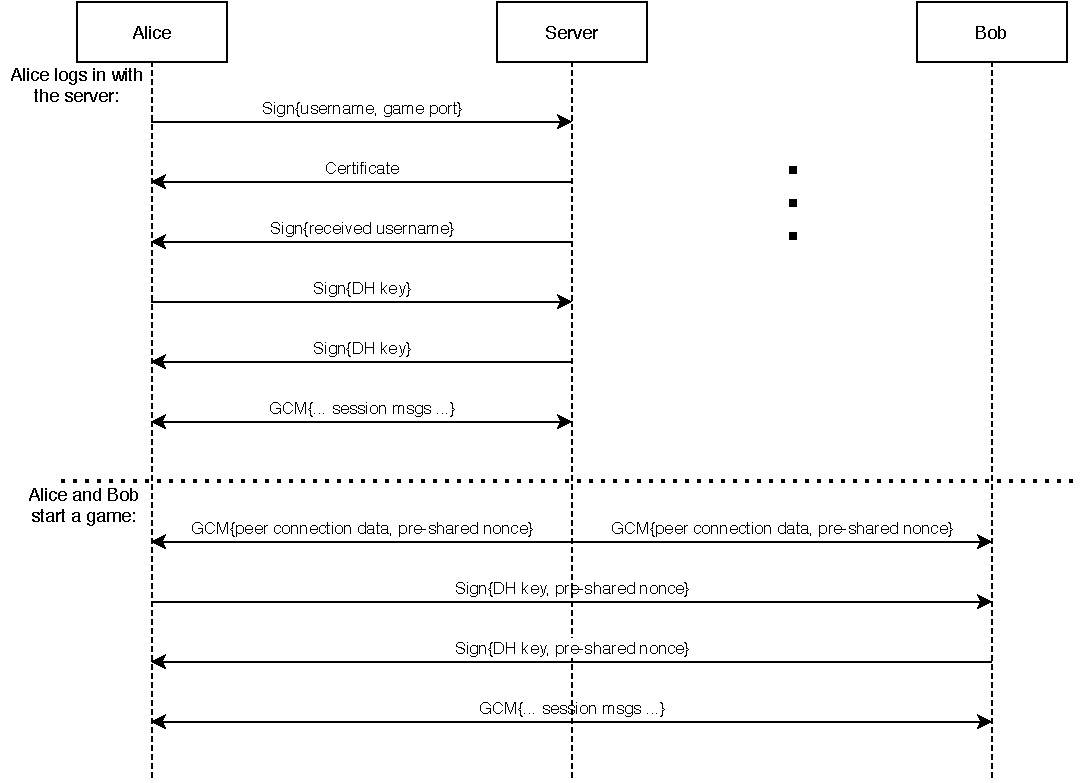
\includegraphics[width=\textwidth]{keyxchng}
	\caption{Sequence diagram of a sample session}\label{fig:keyxchng}
\end{figure}

In the figure only the content of the body part of messages are represented: the
header for each message is always the one shown in \lstref{lst:msgheader}.

\subsection{Formal description}\label{subsec:formal}

In the following we will simplify the protocol messages to only contains the
informations needed to guarantee the security of the protocol (in the real
protocol, each field of the header is always included even when it is not
useful).

\subsubsection{Notation}

\begin{itemize}
	\item \(A\) is a client, also named ``Alice'';
	\item \(B\) is another client, also named ``Bob'';
	\item \(S\) is the server;
	\item \(\mathit{CA}\) is the certification authority;
	\item \(N_P^n\) is a random nonce generated by the principal \(P\). The
		superscript \(n\) is used to distinguish between different
		nonces;
	\item \(\hash(X)\) means ``the hash of \(X\)'';
	\item \(\hash(\ldots)\) means ``the hash of the current message''. So,
		when we write \(\sign{\hash(\ldots)}{K}\) we mean that the
		message is hashed and then the hash is signed with \(K\).
		This represents the work done by the EVP API of \openssl;
	\item \(\mathit{DHKEY}_P^{PQ}\) is the Diffie-Hellman public key
		generated by the principal \(P\) for use in the communication
		between \(P\) and \(Q\);
	\item \(\mathit{DH}_{params}\) are the Diffie-Hellman pre-shared
		parameters (\(p\) and \(g\));
	\item \(K_{GCM}^{PQ}\) is the shared GCM key between \(P\) and \(Q\)
		derived from the shared secret obtained from Diffie-Hellman.
\end{itemize}

\subsubsection{Idealized protocol}

Here we assume that there are no errors and the client successfully
authenticates with the server:
\begin{itemize}
	\item[M1:] \(A \sends S \qquad \sign{N_A^1, A, port}{K_A}\)
	\item[M2:] \(S \sends A \qquad N_S^1, \sign{K_S}{K_{CA}}, \hash(M1)\)
	\item[M3:] \(S \sends A \qquad N_S^2, A, \hash(M1), \sign{\hash(\ldots)}{K_S}\)
	\item[M4:] \(A \sends S \qquad N_A^2, \mathit{DHKEY}_A^{AS}, \hash(M3), \sign{\hash(\ldots)}{K_A}\)
	\item[M5:] \(S \sends A \qquad N_S^3, \mathit{DHKEY}_S^{AS}, \hash(M4), \sign{\hash(\ldots)}{K_S}\)
\end{itemize}

At this point the session key for GCM is derived (\(K_{GCM}^{AS}\)). Here we will
show the continuation of the protocol when Alice asks to challenge Bob. For
simplicity, we do not show the message that the server sends to Bob with the
challenge request and the response for accepting/refusing it (like if the
challenge is automatically accepted by Bob):
\begin{itemize}
	\item[M6:] \(A \sends S \qquad \encrypt{N_A^3, \mathit{CHALL\_REQ}, B, \hash(M5)}{K_{GCM}^{AS}}\)
	\item[M7:] \(S \sends A \qquad \encrypt{N_S^4, \mathit{address}_B, K_B, N_{DH}, \hash(M6)}{K_{GCM}^{AS}}\)
	\item[M8:] \(S \sends B \qquad \encrypt{N_S^5, \mathit{address}_A, K_A, N_{DH}, \hash(\mathit{prev\,msg\,from\,B})}{K_{GCM}^{BS}}\)
	\item[M9:] \(A \sends B \qquad N_A^4, \mathit{DHKEY}_A^{AB}, N_{DH}, \sign{\hash(\ldots)}{K_A}\)
	\item[M10:] \(B \sends A \qquad N_B^1, \mathit{DHKEY}_B^{AB}, N_{DH}, \hash(M9), \sign{\hash(\ldots)}{K_B}\)
	\item[M11:] \(A \sends B \qquad \encrypt{N_A^5, \mathit{GAME\_MOVE}_A, \hash(M10)}{K_{GCM}^{AB}}\)
	\item[M12:] \(B \sends A \qquad \encrypt{N_B^2, \mathit{GAME\_MOVE}_B, \hash(M11)}{K_{GCM}^{AB}}\)
\end{itemize}

\subsubsection{Assumptions}

\begin{itemize}
	\item \(A \believes \fresh{N_A^n}\) for each \(n \in \mathbb{N}\)
	\item \(B \believes \fresh{N_B^n}\) for each \(n \in \mathbb{N}\)
	\item \(S \believes \fresh{N_S^n}\) for each \(n \in \mathbb{N}\)
	\item \(A \believes S \controls N_S^n\) for each \(n \in \mathbb{N}\)
	\item \(B \believes S \controls N_S^n\) for each \(n \in \mathbb{N}\)
	\item \(S \believes A \controls N_A^n\) for each \(n \in \mathbb{N}\)
	\item \(S \believes B \controls N_B^n\) for each \(n \in \mathbb{N}\)
	\item \(A \believes B \controls N_B^n\) for each \(n \in \mathbb{N}\)
	\item \(B \believes A \controls N_A^n\) for each \(n \in \mathbb{N}\)
	\item \(S \believes \fresh{N_{DH}}\)
	\item \(A \believes S \controls N_{DH}\)
	\item \(B \believes S \controls N_{DH}\)
	\item \(S \believes \pubkey{K_A} A\)
	\item \(S \believes \pubkey{K_B} B\)
	\item \(A \believes \pubkey{K_{CA}} \mathit{CA}\)
	\item \(B \believes \pubkey{K_{CA}} \mathit{CA}\)
	\item \(A \believes \mathit{CA} \controls \pubkey{K_S} S\)
	\item \(B \believes \mathit{CA} \controls \pubkey{K_S} S\)
	\item \(A \believes S \controls \pubkey{K_B} B\)
	\item \(B \believes S \controls \pubkey{K_A} A\)
	\item \(A \believes A \secret{\mathit{DH}_{params}} S\)
	\item \(S \believes S \secret{\mathit{DH}_{params}} A\)
	\item \(B \believes B \secret{\mathit{DH}_{params}} S\)
	\item \(S \believes S \secret{\mathit{DH}_{params}} B\)
	\item \(A \believes A \secret{\mathit{DH}_{params}} B\)
	\item \(B \believes B \secret{\mathit{DH}_{params}} A\)
	\item \(A \believes S \controls \mathit{DHKEY}_S^{AS}\)
	\item \(S \believes A \controls \mathit{DHKEY}_A^{AS}\)
	\item \(B \believes S \controls \mathit{DHKEY}_S^{BS}\)
	\item \(S \believes B \controls \mathit{DHKEY}_B^{BS}\)
	\item \(A \believes B \controls \mathit{DHKEY}_B^{AB}\)
	\item \(B \believes A \controls \mathit{DHKEY}_A^{AB}\)
\end{itemize}

\subsubsection{Objectives}

\begin{enumerate}
	\item \(A \believes \pubkey{K_S} S\)
	\item \(B \believes \pubkey{K_S} S\)
	\item \(S \believes \fresh{S \sharedkey{K_{GCM}^{AS}} A}\)
	\item \(A \believes \fresh{A \sharedkey{K_{GCM}^{AS}} S}\)
	\item \(S \believes \fresh{S \sharedkey{K_{GCM}^{BS}} B}\)
	\item \(B \believes \fresh{B \sharedkey{K_{GCM}^{BS}} S}\)
	\item \(A \believes S \believes \fresh{S \sharedkey{K_{GCM}^{AS}} A}\)
	\item \(S \believes A \believes \fresh{A \sharedkey{K_{GCM}^{AS}} S}\)
	\item \(B \believes S \believes \fresh{S \sharedkey{K_{GCM}^{BS}} B}\)
	\item \(S \believes B \believes \fresh{B \sharedkey{K_{GCM}^{BS}} S}\)
	\item \(S \believes A \believes \mathit{CHALL\_REQ}\)
	\item \(A \believes S \believes \mathit{address}_B, K_B, N_{DH}\)
	\item \(B \believes S \believes \mathit{address}_A, K_A, N_{DH}\)
	\item \(A \believes \pubkey{K_B} B\)
	\item \(B \believes \pubkey{K_A} A\)
	\item \(B \believes \fresh{B \sharedkey{K_{GCM}^{AB}} A}\)
	\item \(A \believes \fresh{A \sharedkey{K_{GCM}^{AB}} B}\)
	\item \(A \believes B \believes \fresh{B \sharedkey{K_{GCM}^{AB}} A}\)
	\item \(B \believes A \believes \fresh{A \sharedkey{K_{GCM}^{AB}} B}\)
	\item \(A \believes B \believes \mathit{GAME\_MOVE}_B\)
	\item \(B \believes A \believes \mathit{GAME\_MOVE}_A\)
\end{enumerate}

\subsubsection{Proof}

In M1 the server receive a signed message containing the name \(A\) and the
nonce \(N_A^1\). At this point, the server can verify the signature of the
message but it cannot be sure that the message is fresh.

In M2 Alice receives the server's public key \(K_S\) signed with the public
key of the certification authority. Using the \emph{message meaning rule}:

\[
	\frac{A \believes \pubkey{K_{CA}} \mathit{CA}, A \sees \sign{K_S}{K_{CA}}}%
	{A \believes \mathit{CA} \oncesaid K_S}
\]

Since the CA certifies that \(K_S\) is the public key of \(S\), we can say
that \(A \believes \mathit{CA} \believes \pubkey{K_S} S\). Now, since the
freshness of \(K_S\) is not important (the public key is always the same),
we can apply the \emph{jurisdiction rule}:

\[
	\frac{A \believes \mathit{CA} \believes \pubkey{K_S} S, A \believes \mathit{CA} \controls \pubkey{K_S} S}
	{A \believes \pubkey{K_S} S}
\]

We have proven the (1). The (2) can be proven in the same way.

In M3 Alice receives a message signed with \(K_S\) from \(S\). The
freshness is guaranteed by the fact that the freshness of the nonce sent in M1
(\(A \believes \fresh{N_A^1}\)) implies the freshness of \(\hash(M1)\) (since M1
contains \(N_A^1\)) and this implies the freshness of \(\hash(\ldots)\) which is
signed with \(K_S\). This guarantees Alice that \(S\) has the private key of
\(K_S\): the server has authenticated with the client.

The reasoning done for M3, can be applied to any message \(X\): in fact, if we
are sure about the freshness of \(\hash(\mathit{prev\,msg})\) due to the
freshness of the all previous nonces, we can apply the \emph{nonce verification
rule}:

\[
	\frac{A \believes \fresh{\hash(\mathit{prev\,msg})}, A \believes S \oncesaid \hash(\mathit{prev\,msg})}
	{A \believes S \believes \hash(\mathit{prev\,msg})}
\]

\(A \believes S \oncesaid \hash(\mathit{prev\,msg})\) comes from the
\emph{message meaning rule}:

\[
	\frac{A \believes \pubkey{K_S} S, A \sees \sign{\hash(\ldots)}{K_S}}
	{A \believes S \oncesaid \hash(\ldots)}
\]

And then applying the BAN postulate for hash functions:

\[
	\frac{A \believes S \oncesaid \hash(\ldots), A \sees \ldots}
	{A \believes S \oncesaid \ldots}
\]

Where with \(\ldots\) we mean the entire message, that also contains
\(\hash(\mathit{prev\,msg})\).

Now we are sure that any message between \(A\) and \(S\) (and also between \(B\)
and \(S\)) are correctly authenticated using public key cryptography. This
applies also to messages M4 and M5, which contain the Diffie-Hellman public key.

Thanks to Diffie-Hellman, now we are sure that:

\[
	A \believes A \secret{\mathit{DH}_{secret}} S
\]
\[
	S \believes S \secret{\mathit{DH}_{secret}} A
\]
\[
	A \believes S \believes S \secret{\mathit{DH}_{secret}} A
\]
\[
	S \believes A \believes A \secret{\mathit{DH}_{secret}} S
\]

Since we extract the GCM key from \(\mathit{DH}_{secret}\), we have proven
objectives (3--10).

Now GCM is initialized (M6, M7, M8). Since GCM guarantees confidentiality and
authentication, we have also proven (11), (12), (13).

Since Alice is sure about the identity of \(S\) and his messages are correctly
authenticated thanks to GCM, from the assumption \(A \believes S \controls
\pubkey{K_B} B\) we can apply the \emph{jurisdiction rule}:

\[
	\frac{A \believes S \believes \pubkey{K_B} B, A \believes S \controls \pubkey{K_B} B}
	{A \believes \pubkey{K_B} B}
\]

This proves the (14). The same logic can be applied to prove the (15).

In M7 and M8, \(S\) also sends \(N_{DH}\) to \(A\) and \(B\). Alice and Bob can
assume the freshness of \(N_{DH}\), since they received it from \(S\) that is
now fully trusted. In M9 \(B\) receives \(\mathit{DHKEY}_B^{AB}\) from Alice,
along with \(N_{DH}\), and the same happens in the opposite direction in M10.
Applying the same reasoning done for M1, M2, M3 (\(N_{DH}\) is believed fresh,
as it was for \(N_A^1\) before) we prove (16--19).

Now GCM is initialized for messages M11 and M12. Since GCM guarantees
confidentiality and authentication, we have also proven (20), (21).
